\chapter{Zpracování obrazu}
\label{ch:techniky}
Pro úspěšné vytvoření algoritmu na detekci chorob na sítnici lidského oka je nutné znát jednak konkrétní projevy daných onemocnění, které jsou popsány v~předchozí kapitole, ale také nejrůznější metody zpracování digitálního obrazu. V~této kapitole jsou popsány základní algoritmy z~této oblasti a z~oblasti počítačového vidění.

Máme k~dispozici digitální obraz sítnice. Ten však může být různými způsoby zkreslen (například díky způsobu snímání nebo nevhodným podmínkám při jeho průběhu) a tím pádem nepříznivě ovlivnit detekci. Pro co nejpřesnější a nejlepší výsledky musíme před samotným zahájením procesu detekce provést úpravu tohoto digitálního obrazu. Základní změny, které můžeme provést pro prvotní zpracování obrazu jsou vyhlazování obrazu, prahování a morfologické operace.

\section{Vyhlazování obrazu}
\label{sec:smoothing}
Vyhlazování obrazu používáme pro odstranění nežádoucích artefaktů v~obraze jako je například šum, který může navozovat dojem, jako kdyby obraz zrnil. Existuje mnoho metod pro vyhlazování obrazu, kde každá metoda řeší jiný druh šumu. Tyto metody se také liší svou výpočetní náročností a efektivitou v~odstraňování konkrétního druhu šumu.
\begin{itemize}
  \item \textbf{Průměrování} je konvoluce obrazu s~normalizovanou maskou. Každý pixel překrytý touto maskou vynásobíme koeficientem v~příslušné buňce a provedeme součet všech těchto hodnot. Tím se získá jeden nový pixel. Výšku a šířku této masky lze specifikovat. Konvoluční maska 3$\times$3 by vypadala následovně:
  
  $$
    \text{K} = \frac{1}{9}\left\lbrack
    \begin{array}{ccc}
      1 & 1 & 1\\
      1 & 1 & 1\\
      1 & 1 & 1\\
    \end{array} \right\rbrack
  $$

  \item \textbf{Gaussovo vyhlazování} je jednou z~metod odstranění šumu využívající konvoluce obrazu s~maskou, která se skládá z~elementů určených Gaussovou funkcí. Ty slouží pro výpočet transformací, které se aplikují na každý pixel v~obraze. Gaussovo vyhlazování je velmi efektivní technika v~odstraňování Gaussovského šumu, který odpovídá Gaussovu rozložení. Tento šum si lze prohlédnout na obrázku \ref{pic:chap04_lenna_gauss_noise}. Rovnice Gaussovy funkce ve dvou dimenzích \cite{comp_vision}:

  \begin{equation}
    G(x,y)=\frac{1}{2\pi\sigma^2}e^{-{\frac{x^2+y^2}{2\sigma^2}}}
  \end{equation}

  kde $x$ a $y$ jsou souřadnice v~obraze a $\sigma$ je směrodatná odchylka Gaussovy distribuce. Ukázka Gaussovy matice je zobrazena na obrázku \ref{pic:chap04_gaussian_matrix}.
  
  \begin{figure}[h]
	\begin{center}
		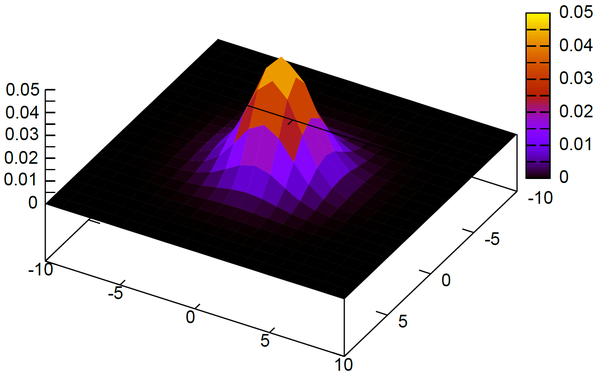
\includegraphics[width=0.75\linewidth]{chap04_gaussian_matrix}
		\caption{Gaussova matice (okolí 10 pixelů, odchylka 1,8) \cite{pic_gauss_matrix}.}
		\label{pic:chap04_gaussian_matrix}
	\end{center}
  \end{figure}

  \item \textbf{Mediánové vyhlazování} vymezí pro každý pixel obrazu jeho okolí. Ze všech těchto pixelů vybere medián, který se stává novou hodnotou zpracovávaného pixelu. To je vysoce účinné pro odstraňování šumu typu sůl a pepř, který je viditelný na obrázku \ref{pic:chap04_lenna_salt_pepper}. Ve výše uvedených filtrech je centrálním prvkem nově vypočtená hodnota, která může být existující hodnotou pixelu v~obraze nebo zcela novou hodnotou. Při mediánovém vyhlazování je centrální prvek vždy nahrazen hodnotou nějakého pixelu v~obraze.
  
  \begin{figure}[h]
    \begin{minipage}[c]{0.47\textwidth}
      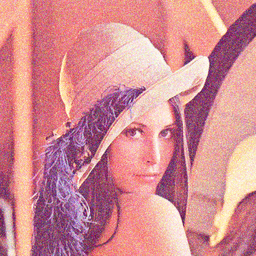
\includegraphics[width=\linewidth]{chap04_lenna_gauss_noise}
      \caption{Gaussovský šum \cite{pic_lenna}.}
      \label{pic:chap04_lenna_gauss_noise}
    \end{minipage}
    \hfill
    \begin{minipage}[c]{0.47\textwidth}
      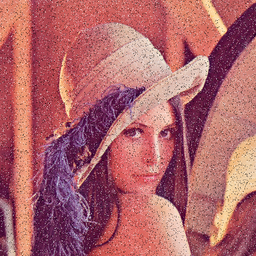
\includegraphics[width=\linewidth]{chap04_lenna_salt_pepper}
      \caption{Šum typu sůl a pepř.}
      \label{pic:chap04_lenna_salt_pepper}
    \end{minipage}
  \end{figure}

\end{itemize}

\section{Prahování}
Prahování neboli tresholding je nejjednodušší metoda segmentace digitálního obrazu založená na hodnocení intenzity jednotlivých pixelů. Jejím principem je nalezení takové hodnoty prahu (threshold), pro kterou bude platit, že všechny hodnoty intenzity vyšší než práh odpovídají popředí, zatímco všechny hodnoty nižší než práh odpovídají pozadí. V~případě, že se rozložení intenzity pixelů popředí a pozadí výrazně překrývá, může být nalezení vhodné hodnoty prahu prakticky nemožné. Z~obrázku ve stupních šedi lze prahováním vytvořit binární (černobílý) obraz. Je to metoda jednoduchá a rychlá, ale relativně destruktivní pro výsledný obraz. Binární prahování lze vyjádřit následujícím vztahem \cite{izg}:
\begin{equation}
  P(x,y) = \left\{
  \begin{array}{l l}
    1 & \text{pro} \quad I(x,y) \geq T\\
    0 & \text{pro} \quad I(x,y) < T
  \end{array} \right.
\end{equation}

\textbf{Adaptivní prahování} je možné využít v~případech, kdy má zpracovávaný obraz odlišné světelné podmínky v~různých oblastech, což znemožňuje přímo určit jeden globální práh. Tato metoda rozdělí obraz na menší části, pro každou vypočte prahovou hodnotu a následně provede binární prahování jednotlivých oblastí. Tímto způsobem se docílí lepších výsledků u~obrazů s~různým osvětlením. Rozdíl mezi binárním a adaptivním prahováním lze pozorovat na obrázcích \ref{pic:chap04_lenna_thresh_bin} a \ref{pic:chap04_lenna_thresh_ada}.

\begin{figure}[h]
  \begin{minipage}[c]{0.47\textwidth}
    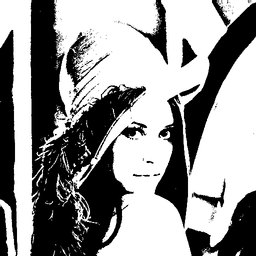
\includegraphics[width=\linewidth]{chap04_lenna_thresh_binary}
    \caption{Binární prahování s~globálním prahem.}
    \label{pic:chap04_lenna_thresh_bin}
  \end{minipage}
  \hfill
  \begin{minipage}[c]{0.47\textwidth}
    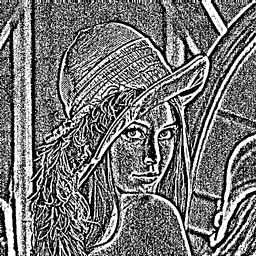
\includegraphics[width=\linewidth]{chap04_lenna_thresh_adaptive}
    \caption{Adaptivní Gaussovo prahování.}
    \label{pic:chap04_lenna_thresh_ada}
  \end{minipage}
\end{figure}

\textbf{Distribuce chyby} je další metoda převodu obrazu ve stupních šedi na černou a bílou, která je v~základu založena na metodě prahování. K~tomu je přidána distribuce vznikajících chyb okolním, dosud nezpracovaným pixelům. Je-li aktuální pixel převeden na černý, pak se vzniklá chyba rovná původní hodnotě pixelu. Je-li aktuální pixel převeden na bílou, pak se vzniklá chyba rovná rozdílu maximální hodnoty obrazu a původní hodnoty pixelu \cite{izg}.

\pagebreak
\section{Morfologické operace}
Matematická morfologie vychází z~vlastností bodových množin. Nejčastěji se aplikuje na binární obrazy, ale lze ji snadno zobecnit i na šedotónové a barevné obrazy. Morfologické operace se používají pro předzpracování (odstranění šumu, zjednodušení tvaru objektů), zdůraznění struktury objektů (kostra, ztenčování, zesilování, konvexní obal, označování objektů) a pro popis objektů číselnými charakteristikami (plocha, obvod, projekce, atd.).

Morfologické operace jsou realizovány jako relace obrazu (bodové množiny X) s~jinou menší bodovou množinou B, tzv. strukturním elementem. Morfologickou transformaci si lze představit jako určitý systematický pohyb strukturního elementu B po obrazu X a vyhodnocení odezvy podle typu operace. Mezi dvě základní morfologické operace patří dilatace a eroze.

\textbf{Dilatace} skládá body dvou množin pomocí vektorového součtu. Objekty v~obraze jsou po aplikaci dilatace zvětšené na úkor pozadí. Dilatace se používá k~zaplnění děr popř. zálivů a její definiční vztah je dán následujícím vzorcem \cite{feec}:

\begin{equation}
X \oplus B = \{d \in E^2 : d = x + b, x \in X, b \in B\}
\end{equation}

\textbf{Eroze} skládá dvě bodové množiny s~využitím vektorového rozdílu. Je duální (nikoliv inverzní) transformací k~dilataci a používá se pro zjednodušení struktury objektů. Objekty jednotkové tloušťky (relativní jednotka) zmizí a složité objekty spojené čárami jednotkové tloušťky se rozloží na několik jednodušších objektů. Eroze je dána následujícím vzorcem \cite{feec}:

\begin{equation}
X \Theta B = \{d \in E^2 : d + b \in X \text{ pro } \forall b \in B\}
\end{equation}

  \begin{figure}[h]
	\begin{center}
		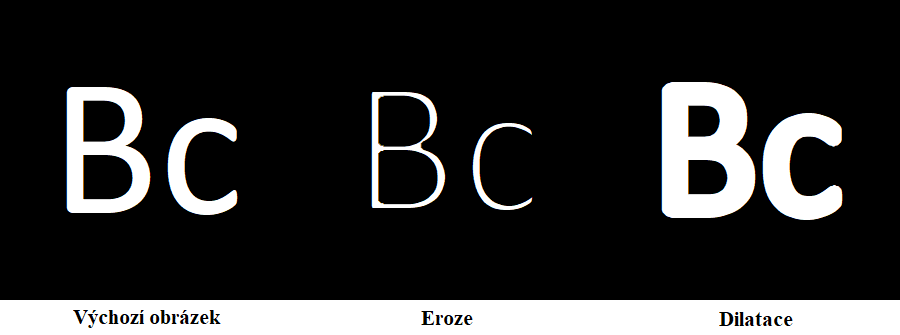
\includegraphics[width=.75\linewidth]{chap04_morph_overview}
		\caption{Základních morfologické operace.}
		\label{pic:chap04_morph_overview}
	\end{center}
  \end{figure}

Další morfologické operace jsou \textbf{otevření} a \textbf{uzavření} a jsou to operace, které vzniknou vzájemnou kombinací elementárních operací dilatace a eroze. Výsledkem obou je zjednodušený obraz, který obsahuje méně detailů (odstraní detaily menší než strukturní element, celkový tvar objektu se ale neporuší). Eroze následovaná dilatací se nazývá morfologické otevření, které je viditelné na obrázku \ref{pic:chap04_morph_open}. To oddělí objekty spojené úzkou šíjí, a tak zjednoduší strukturu objektů. Na obrázku \ref{pic:chap04_morph_close} je zobrazena dilatace následovaná erozí, která se naopak nazývá morfologické uzavření. Ta spojí objekty, které jsou blízko u~sebe, zaplní díry a vyhladí obrys \cite{feec}.

  \begin{figure}[h]
  \begin{minipage}[c]{0.47\textwidth}
    
\includegraphics[width=\linewidth]{chap04_morph_open}
		\caption{Morfologické otevření.}
		\label{pic:chap04_morph_open}
  \end{minipage}
  \hfill
  \begin{minipage}[c]{0.47\textwidth}
    
\includegraphics[width=\linewidth]{chap04_morph_close}
		\caption{Morfologické uzavření.}
		\label{pic:chap04_morph_close}
  \end{minipage}
\end{figure}

\pagebreak
\section{Momenty}
V~oblasti zpracování obrazu, počítačového vidění a souvisejících oborů je obrazový moment určitým váženým průměrem intenzity obrazových pixelů nebo funkcí takových momentů, obvykle vybraných tak, aby měly nějakou atraktivní vlastnost nebo interpretaci. Obrazové momenty jsou užitečné při popisu objektů po segmentaci. Jednoduché vlastnosti obrazu, které jsou pomocí nich získány, zahrnují oblast (nebo celkovou intenzitu), její těžiště a informace o~její orientaci. V~případě obrazu v~odstínech šedi a s~intenzitou pixelů $I(x,y)$ se momenty obrazu $M_{ij}$ vypočítají pomocí vztahu \cite{img_moments}:

\begin{equation}
M_{ij} = \sum_{x}\sum_{y} x^i y^j I(x,y)
\end{equation}

\noindent a následně můžeme vypočítat těžiště dané oblasti:

\begin{equation}
x = \frac{M_{10}}{M_{00}} \quad \text{a} \quad y = \frac{M_{01}}{M_{00}}
\end{equation}

\section{Houghova transformace}
Jedná se o~techniku extrakce vlastností. Jejím účelem je nalézt nedokonalé instance objektů v~rámci určité třídy tvarů pomocí hlasování. To se provádí v~prostoru parametrů, ze kterého jsou kandidáti objektů získání jako lokální maxima v~tzv. akumulačním prostoru, který je explicitně zkonstruován algoritmem při výpočtu Houghovy transformace. Klasická Houghova transformace byla určena pro identifikaci přímek v~obraze, ale později byla rozšířena pro určení pozic libovolných tvarů, nejčastěji kruhů nebo elips \cite{comp_vision}.

\section{Semínkové vyplňování}
Semínkové nebo také záplavové vyplňování slouží pro vyplnění dané oblasti ohraničené nějakým uzavřeným polygonem. Ze znalosti vnitřního bodu se určí, zda sousední body leží uvnitř oblasti nebo na její hranici. Podle způsobu určování sousedních bodů máme dva způsoby vyplňování, a to metodu používající čtyř sousedních bodů a metodu používající osmi sousedních bodů.

\subsection*{Algoritmus semínkového vyplňování}
Tento algoritmus má tři parametry: počáteční bod, hledanou barvu a cílovou barvu. Algoritmus vyhledá všechny body v~oblasti, které jsou připojeny k~počátečnímu bodu cestou hledané barvy, a změní je na cílovou barvu.
  \begin{enumerate}
    \item Pokud je barva bodu rovna cílové barvě, skonči.
    \item Pokud je barva bodu jiná než hledaná barva, skonči.
    \item Nastav barvu bodu na cílovou barvu.
    \item Znovu použij tento algoritmus pro všechny sousední body.
  \end{enumerate}
